\documentclass[a4paper,11pt]{article}

\usepackage{times}
%\setcounter{secnumdepth}{0} % sections are not getting numbered
\usepackage[english,serbian]{babel}


\usepackage[T1]{fontenc} 
%\usepackage[backend=biber,style=numeric,sortcites,sorting=nty,backref,natbib,hyperref]{biblatex} % bibliography

%\addbibresource{citation.bib} % file with references


\usepackage{comment}
\usepackage{amsfonts}
\usepackage{amsmath}
\usepackage{amsthm}
\usepackage{IEEEtrantools}
\usepackage{graphicx}
%\usepackage{cite}

%\usepackage{geometry}
%\usepackage{upgreek}
\usepackage[serbian]{babel}
%\usepackage{ulem}
%\usepackage{environ}
\usepackage{tikz}
\usepackage{color}
\usepackage{fancybox}

%\numberwithin{equation}{section}
\theoremstyle{definition} \newtheorem{deff}{Definicija}[section]
\theoremstyle{definition} \newtheorem{prim}[deff]{Primer}
\theoremstyle{plain} \newtheorem{teor}[deff]{Teorema}


\newcommand{\unija}[2]{#1 \cup #2}
\newcommand{\pres}[2]{#1 \cap #2}
\newcommand{\tnorm}{$t$-norm}
\newcommand{\tkonorm}{$t$-konorm}
\newcommand{\vect}[1]{\boldsymbol{\mathbf{#1}}}

\renewenvironment{proof}[1][\proofname]{{\bfseries #1.}}

\frenchspacing


\usepackage[a4paper,top=3cm,bottom=2cm,left=2cm,right=2cm,marginparwidth=1.75cm]{geometry}
%% Useful packages
\usepackage{mathrsfs}
\newsavebox\foobox
\newlength{\foodim}
\newcommand{\slantbox}[2][0]{\mbox{%
		\sbox{\foobox}{#2}%
		\foodim=#1\wd\foobox
		\hskip \wd\foobox
		\hskip -0.5\foodim
		\pdfsave
		\pdfsetmatrix{1 0 #1 1}%
		\llap{\usebox{\foobox}}%
		\pdfrestore
		\hskip 0.5\foodim
}}
\def\Laplace{\slantbox[-.45]{$\mathscr{L}$}}

%\usepackage[colorinlistoftodos]{todonotes}

\usepackage{caption}
\usepackage{subcaption}
\usepackage{changepage}
\usepackage{multirow}

\usepackage{blindtext}

\usepackage{tabularx}
\usepackage[export]{adjustbox}

\usepackage[utf8]{inputenc}
\usepackage[T1]{fontenc}
\usepackage{lmodern}
\usepackage{graphicx}
\usepackage{color}
\usepackage{listings}
\usepackage{amsmath}

%\usepackage[usenames,dvipsnames]{xcolor}
%\usepackage[colorlinks=true,linkcolor=blue]{hyperref}

\usepackage{amsfonts}
\usepackage{epstopdf}

\usepackage{float}

\usepackage[shortlabels]{enumitem}
\usepackage[yyyymmdd]{datetime}


\renewcommand{\figurename}{Slika}

\DeclareMathOperator*{\argmax}{\arg\max}
\graphicspath{{./images/}}

\usepackage{booktabs}

\usepackage{siunitx}

\usepackage{scalerel}






\sloppy

\epstopdfsetup{update} % only regenerate pdf files when eps file is newer

%%%%%%%% DOCUMENT %%%%%%%%
\setlength {\marginparwidth }{2cm}
\begin{document}
	
	%%%% Title Page
	\begin{titlepage}
		
		\newcommand{\HRule}{\rule{\linewidth}{0.5mm}} 							% horizontal line and its thickness
		\center 
		
		% University
		\textsc{\LARGE Elektrotehnički fakultet u Beogradu}\\[1cm]
		
		% Document info
		\textsc{\Large Distribuirani i frakcioni sistemi upravljanja}\\[0.2cm]
		\textsc{\large 13M051DIF}\\[1cm] 										
		\HRule \\[0.8cm]
		{ \huge \bfseries Projektovanje kontrolera primenom analiti"ckih i optimizacionih tehnika }\\[0.7cm]								% Assignment
		%\HRule \\[2cm]
		
		
		\large
		\vfill 
		\emph{Studenti:}\\
		Nikita Jokić 3279/2023\\[0.1cm]
		\emph{Mentor:}\\
		prof. dr Tomislav "Sekara\\[0.1cm]									
		{\large 2024}\\[2cm]
	\end{titlepage}
	\tableofcontents
	\newpage
	
	\section{Modeliranje sistema i projektovanje kontrolera}\label{sec:mod i projektovanje}
	\subsection{Uvod} 
	
	Stabilnost frekvencije u elektroenergetskim sistemima jedan je od ključnih faktora za obezbeđivanje sigurnog i efikasnog rada, kako u normalnim, tako i u izuzetnim uslovima. Naime, frekvencijska devijacija, koja može biti izazvana promenama u opterećenju, kvarovima ili spoljnim poremećajima, utiče ne samo na rad električnih mašina, već i na ukupne performanse sistema, uključujući sigurnost prenosa električne energije. U slučaju značajnijih odstupanja od nominalne frekvencije, dolazi do preopterećenja sistema, što može izazvati lančane reakcije koje potencijalno vode ka kvarovima ili čak isključenju delova mreže. \\
	
	U svetlu ovih izazova, dizajn kontrolera za regulaciju frekvencije predstavlja jednu od najvažnijih tema u savremenoj elektroenergetici. Ovaj rad se fokusira na analizu i primenu različitih pristupa projektovanju kontrolera koji mogu efikasno potisnuti frekvencijske devijacije i stabilizovati sistem. Razmatraju se dve osnovne tehnike: analitičko projektovanje kontrolera i optimizacija, pri čemu svaka od ovih metoda ima svoje prednosti i nedostatke u pogledu složenosti, performansi i robusnosti. \\
	
	Analitičko projektovanje kontrolera polazi od preciznog matematičkog modela sistema. Ovaj pristup omogućava tačnu analizu i dizajn sistema, ali ima određena ograničenja kada se sistem nalazi pod promenljivim uslovima, kao što su varijacije u opterećenju ili prisustvo šuma u merenjima. Postoje i druge moderne tehnike projektovanja, kao što su optimizacione metode, koje uzimaju u obzir dinamiku sistema i omogućavaju projektovanje u skladu sa ograni"cenjem robustnosti i merom performansi.\\
	
	Kroz ovaj rad je analizirana primena ovih tehnika za regulaciju frekvencije u modelu elektroenergetskog sistema koji obuhvata parnu turbinu, generator i regulator. Modeliranje sistema vršeno je u Simulink okruženju, pri čemu su parametri sistema, kao što su vremenske konstante generatora, turbine i regulatora, uzeti u obzir prilikom verifikacije kontrolera. Ove konstante igraju ključnu ulogu u odgovoru sistema na poremećaje, jer utiču na brzinu stabilizacije frekvencije i potiskivanje poremećaja u mreži.\\
	
	Jedan od izazova sa kojima se suočava projektovanje kontrolera u ovakvim sistemima je obezbeđivanje da kontroler ne samo da eliminiše devijacije u nominalnim uslovima, već i da ostane stabilan pri promenama parametara sistema. U analitičkom pristupu, dizajn kontrolera bazira se na matematičkim jedna"cinama koje opisuju dinamiku sistema, dok optimizacioni pristup omogućava odre\dj{}ivanje parametara kontrolera tako da posti"zu optimalne performanse.\\
	
	Na kraju, kroz ovaj rad se sprovodi komparativna analiza između analitički projektovanih PID kontrolera i onih dobijenih optimizacijom. Rezultati simulacija, koje su sprovedene u nominalnim i varijabilnim uslovima, prikazuju kako različite tehnike projektovanja utiču na stabilnost, robusnost i efikasnost sistema, te pružaju uvid u optimalne strategije za regulaciju frekvencije u savremenim elektroenergetskim mrežama.\\
	
	
	
	\newpage
	
	\subsection{Modeliranje sistema}\label{sec:modeliranje}
	
	Modeli su ključni elementi u projektovanju kontrolera jer omogućavaju simulaciju sistema i testiranje kontrolera u preliminarnoj fazi, u offline režimu. U slučaju modernih elektroenergetskih sistema postoji potreba za regulacijom frekvencije u mre"zi, odnosno potiskivanjem devijacija od nominalne frekvencije. 
	Na slici (Sl. \ref{fig:lin_model}) je predstavljen upro"s\'ceni model razmatranog sistema. U tabeli \ref{tab:parametri} su opisani parametri koji se koriste u modelu. \cite{inicijalna}\\
	
	
	\begin{figure}[!htb]
		\centering
		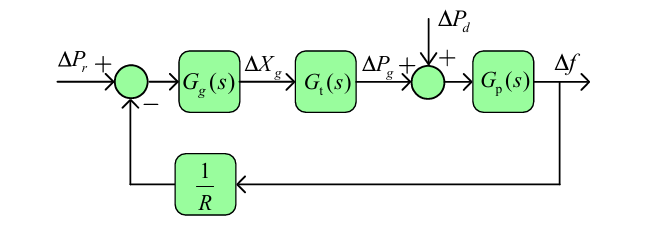
\includegraphics[width=\linewidth]{slike/lin_model.png}
		
		\caption{Upro"s\'cen blok dijagram linearizovanog elektroenergetskog sistema za potrebe regulacije frekvencije, preuzeto iz \cite{inicijalna} \label{fig:lin_model}}
	\end{figure}
	
	
	
	\begin{table}[]
		\resizebox{\textwidth}{!}{%
			\begin{tabular}{lll}
				\hline
				Notacija         & Zna"cenje                                               & Merna jedinica \\ \hline
				T$_G$            & Vremenska konstanta regulatora                          & s              \\
				R                & Regulacija brzine                                       & Hz/p.u. MW     \\
				T$_T$            & Vremenska konstanta turbine                             & s              \\
				T$_P$            & Vremenska konstanta generatora                          & s              \\
				K$_P$            & Poja"canje elektri"cnog sistema                         & -              \\
				$\Delta$f(t)     & Devijacija frekvencije od nominalne vrednosti           & Hz             \\
				$\Delta$P$_r$(t) & Referentno optere\'cenje                 & p.u. MW        \\
				$\Delta$P$_g$(t) & Inkrementalna promena izlaza generatora                 & p.u. MW        \\
				$\Delta$X$_g$    & Inkrementalna promena pozicije ventila regulatora       & -              \\
				$\Delta$P$_d$    & Poreme\'caj optere\'cenja & p.u. MW        \\ \hline
			\end{tabular}%
		}
	\caption{Tabela parametara}
	\label{tab:parametri}
	\end{table}
	
	Razmatrani model se sastoji od 3 glavne komponente: 
	\begin{itemize}
		\item Regulator brzine protoka pare u turbinu $G_g(s)$ , regulacije se vr"si pode"savanjem pozicije ventila. $G_g(s) = \frac{1}{T_Gs+1}$
		\item Parna turbina $G_t(s)$, kovertuje energiju pare u rotacionu energiju. $G_t(s) = \frac{1}{T_Ts+1}$
		\item Generator i dinamika optere\'cenja se modeluju kao jedan sistem $G_p(s) = \frac{K_P}{T_Ps + 1}$, gde je $K_P = \frac{1}{D}$ i $T_P = \frac{2H}{D}$. Koeficijent $H$ je konstanta inercije, opisuje inerciju energije u rotoru. Koeficijent $D$ je prigu"senje optere\'cenja, tipi"cno je u opsegu 1-2.
	\end{itemize}
	
	U radu \cite{inicijalna} kao re"senje za regulaciju devijacije frekvencije se predla"ze uvo\dj{}enje dodatne povratne sprege. Pri "cemu se vodi ra"cuna o tome da se poni"sti uticaj unutra"snje povratne sprege usvajanjem slede\'ce strukture kontrolera: $Q(s) - \frac{1}{R}$. Na slici (Sl. \ref{fig:kontroler_model}) je prikazana predlo"zena struktura upravljanja. 
	
	
	\begin{figure}[!htb]
		\centering
		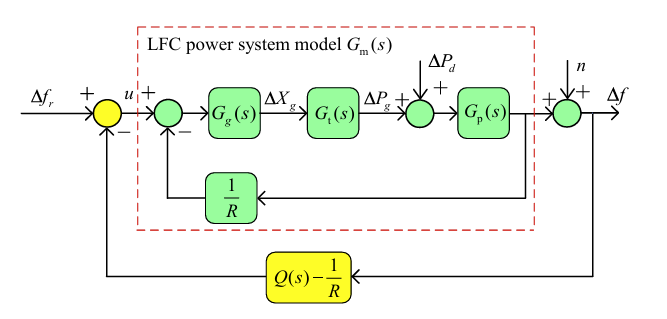
\includegraphics[width=\linewidth]{slike/kontroler_model.png}
		
		\caption{Struktura upravljanja sa kontrolerom $Q(s) - \frac{1}{R}$, preuzeto iz \cite{inicijalna}}
		\label{fig:kontroler_model}
	\end{figure}
	
	Poni"stavanje dinamike unutra"snje povratne sprege za rezultat ima to da se kontroler $Q(s)$ projektuje za sistem $G(s) = G_g(s)G_t(s)G_p(s)$, tj. karakteristi"cni polinom ovog sistema je $1+Q(s)G(s)$. Cilj dizajna kontrolera u narednim sekcijama je odrediti zakon upravljanja koji posti"ze nultu gre"sku u stacionarnom stanju devijacije frekvencije, kao i da se efikasno potisne uticaj poreme\'caja optere\'cenja. Prilikom projektovanja treba uzeti u obzir indikatore performanse i stabilnosti.  \\
	
	
	\subsubsection{Simulink model}\label{sec:matlab_model}
	
	Za potrebe verifikacije projektovanih kontrolera implementiran je kontinualni model u Simulink programskom paketu. Za korak simulacije je usvojeno $T_s = 500~\unit{\mu s}$, ovaj izbor je adekvatan zato "sto su sve vremenske konstante u modelu ve\'ce za bar 2 reda veli"cine.
	
	\begin{figure}[!htb]
		\centering
		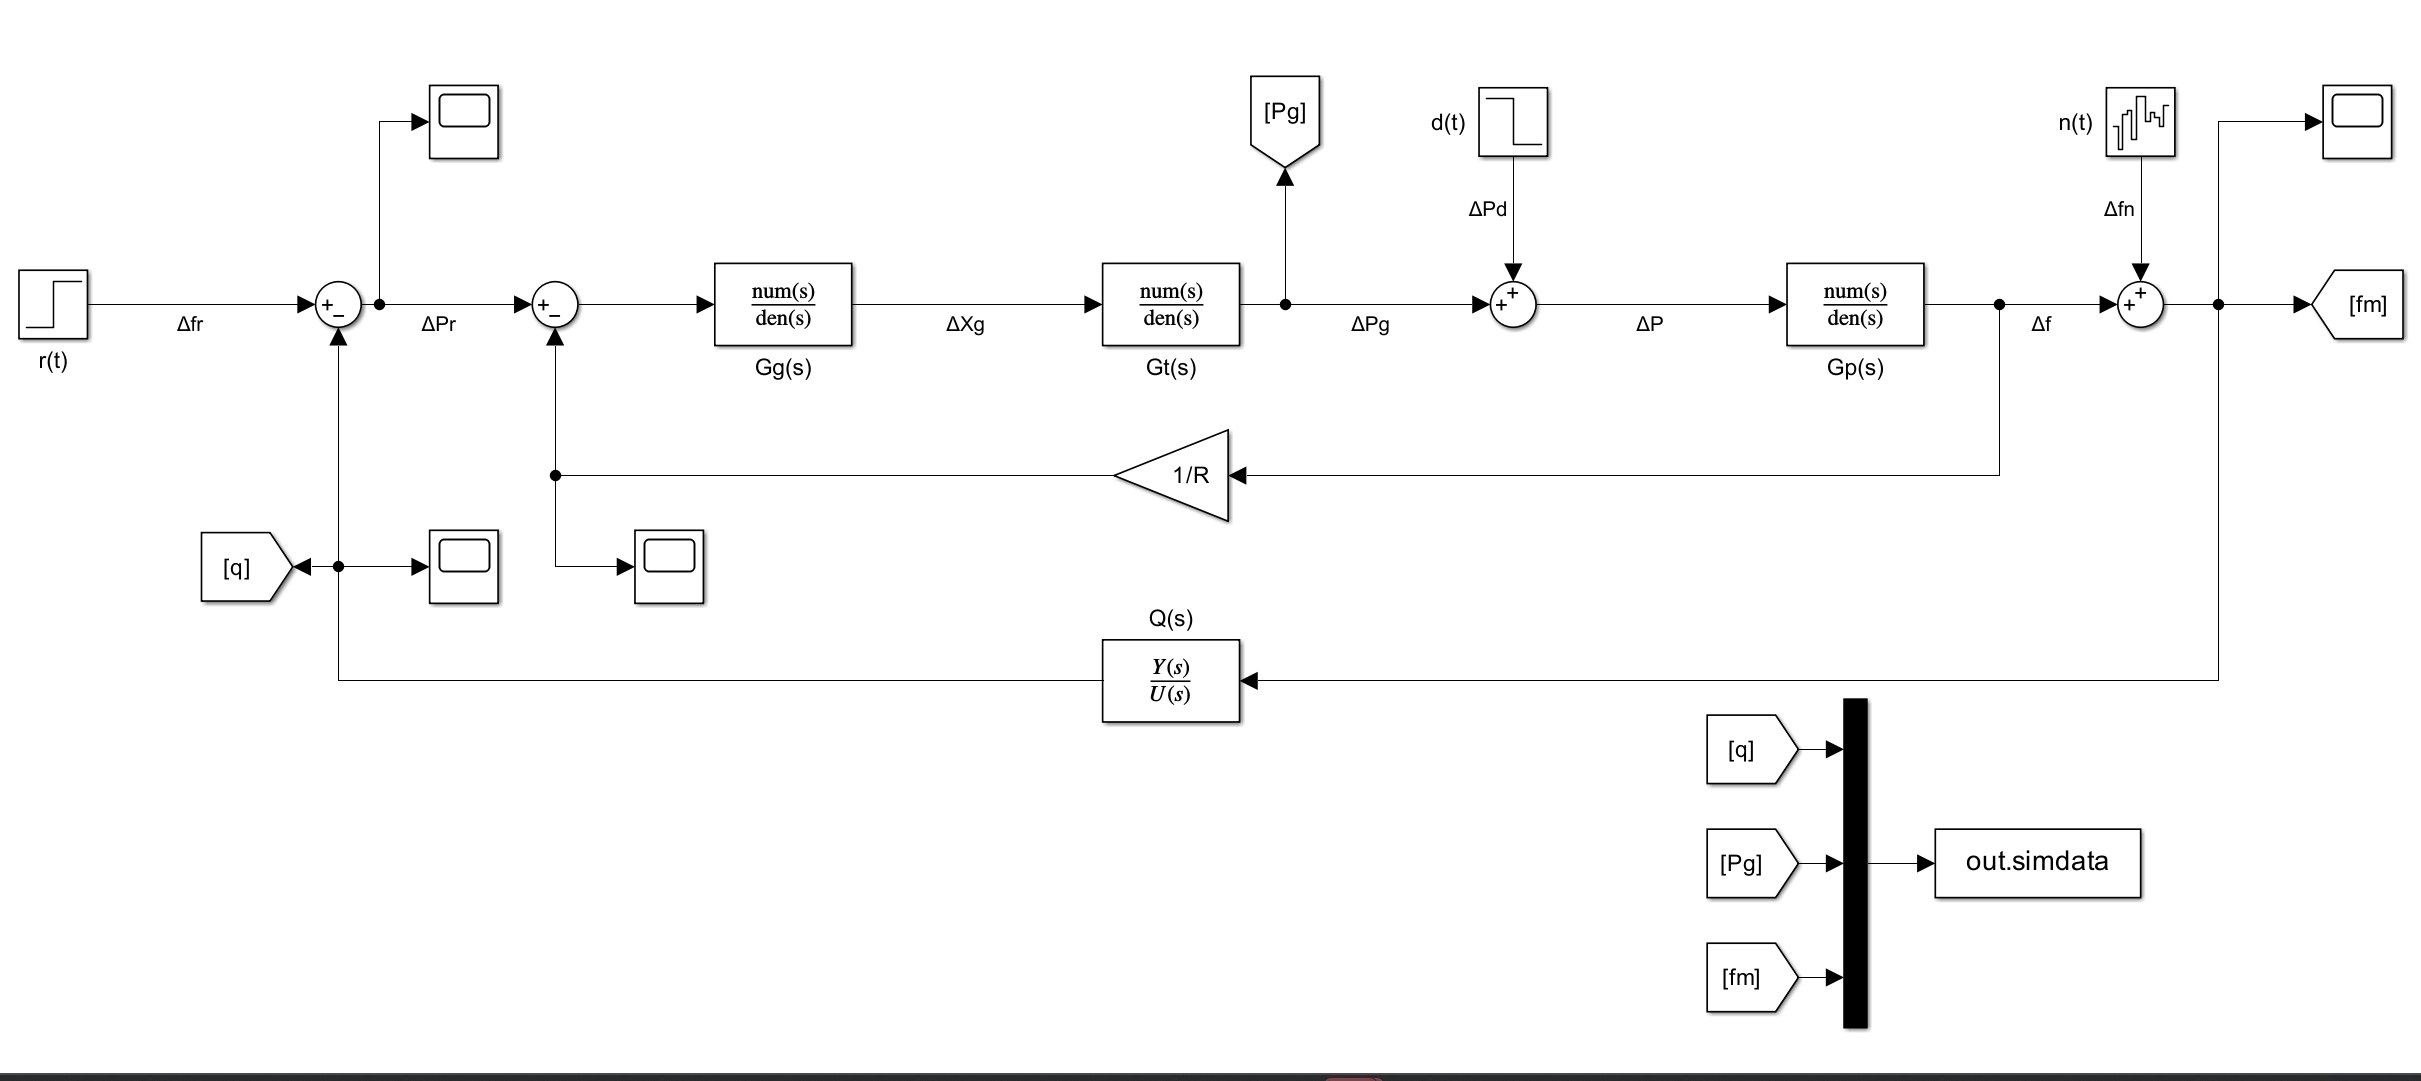
\includegraphics[width=.8\linewidth]{slike/model.png}
		\label{fig:model}
	\end{figure}
	
	\clearpage
	
	\subsection{Projektovanje kontrolera}\label{sec:projektovanje kont}
	
	U ovoj sekciji se opisuju metode kori"\'cene za projektovanje kontrolera "ciji je zadatak da potisnu devijaciju frekvencije od niminalne vrednosti. Kao "sto je napomenuto u sekciji (\ref{sec:modeliranje}) kontroler ima formu $Q(s) - \frac{1}{R}$, a karakteristi"cni polinom sistema je oblika $1+Q(s)G(s)$. Prilikom projektovanja koriste se moderne tehnike koje istovremeno uzimaju u obzir indikatore performansi i robustnosti. Metrike performanse se mogu definisati u vremenskom i frekvencijskom domenu.\\
	
	Va"znije metrike performanse u vremenskom domenu su slede\'ce \cite{inicijalna}: 
	\begin{itemize}
		\item Integral apsolutne gre"ske (IAE) se koristi kao mera potiskivanja poreme\'caja:
		\begin{equation}
			\operatorname{IAE} = \int_{0}^{+\infty}|\Delta f_{\Delta P_d}(t)|~\operatorname{d}t, 
		\end{equation}
		gde je $\Delta f_{\Delta P_d}(t)$ odziv sistema na jedini"cni step poreme\'caj. 
		
		\item Ote"zinjeni integral apsolutne gre"ske (IT$^\alpha$AE) je alternativna mera potiskivanja poreme\'caja:
		\begin{equation}
			\operatorname{IT^\alpha AE} = \int_{0}^{+\infty}t^\alpha|\Delta f_{\Delta P_d}(t)|~\operatorname{d}t~. 
		\end{equation}
			
		\item Upravlja"cki napor prilikom potiskivanja poreme\'caja se kvantifikuje totalnom varijacijom (TV$_d$) upravlja"ckog signala $u(t)$ prilikom odziva na step poreme\'caj $\Delta P_d(s) = \frac{1}{s}$. Totalna varijacija $u(t)$ defini"se se nad odbircima upravlja"ckog signala kao:
		\begin{equation}
			\operatorname{TV_d} = 
			\sum_{i = 1}^{+\infty} |u_{i+1} - u_i|~.
		\end{equation}
		
	\end{itemize}
	
	U frekvencijskom domenu se defini"su tri metrike \cite{bele"ske}:
	
	\begin{itemize}
		\item Robustnost se posti"ze ograni"cavanjem modula funkcije osetljivosti $S(\omega)$: 
		\begin{equation}
			M_S = \operatorname{max}_{\omega}|\frac{1}{1+C(\omega)G_m(\omega)}| = \operatorname{max}_{\omega}|\frac{1+\frac{G(\omega)}{R}}{1+Q(\omega)G(\omega)}|~.
		\end{equation}

		
		\item Otpornost na nesigurnosti u modelu se posti"ze ograni"cavanjem modula komplementarne funkcije osetljivosti
		$T(\omega) = 1 - S(\omega)$:
		
		\begin{equation}
			M_T = \operatorname{max}_{\omega}|\frac{(Q(\omega) - 1/R)G(\omega)}{1+Q(\omega)G(\omega)}|~.
		\end{equation} 
		
		
		\item Otpornost na merni "sum se posti"ze ograni"cavanjem modula funkcije prenosa od "suma $n$ do upravlja"ckog signala $u$:
		\begin{equation}
			M_n = \operatorname{max}_{\omega}|\frac{-C(\omega)}{1+C(\omega)G_m(\omega)}| = \operatorname{max}_{\omega}|\frac{-Q(\omega) + \frac{1}{R}}{1+Q(\omega)G(\omega)}|~.
		\end{equation}
		
	\end{itemize}
	
	U sekciji (\ref{sec:analiticko_projektovanje}) se projektuje kontroler primenom analiti"ckih metoda. Prvo se projektuje PID$_{c_1}$, a zatim se vr"si linearizacija dobijenog kontrolera u okolini ta"cke $s = 0$ i $s = \frac{1}{\lambda}$. Prednost ovog pristupa je to "sto rezultuju\'ci kontroleri imaju podesive parametre $\lambda$ i $N$.\\
	
	U sekciji (\ref{sec:opt_vr}) i  (\ref{sec:opt_fr}) kontroleri se projektuju optimizacijom u vremenskom i frekvencijskom domenu. Parametri su odabrani tako da budu u skladu sa kontrolerima dobijenih linearizacijom.
	
	\clearpage
	
	
	%\clearpage 
	\subsubsection{Analiti"cko projektovanje}
	\label{sec:analiticko_projektovanje}
	
	Prilikom analiti"ckog projektovanja polazi se od izraza za odziv sistema na poreme\'caj:
	\begin{equation}
		Y_d(s) = \frac{1}{1+Q(s)G(s)}G_{p}(s)D(s) \equiv (1 - W(s))G_{p}(s)D(s)~. 
	\end{equation}
	Idealno potiskivanje poreme\'caja se posti"ze za $W(s) = 1 + 0i$. Me\dj{}utim, specificiranje takve funkcije spregnutog prenosa rezultuje fizi"cki ne ostvarivim kontrolerima. Kao alternativa, za poreme\'caje step prirode, dovoljno je usvojiti $W(0) = 1$. Nakon "sto se specificira "zeljeni oblik funkcije spregnutog prenosa kontroler $Q(s)$ mo"ze se dobiti kao:
	\begin{equation}\label{eq:Q(s)}
		Q(s) = \frac{W(s)}{1-W(s)}\frac{1}{G(s)}~.
	\end{equation}\\
	
	U radu \cite{inicijalna} predlo"zena je slede\'ca forma funckije spregnutog prenosa:
	\begin{equation}\label{eq:W(s)}
		W(s) = \frac{\eta_ss+1}{(\lambda s + 1)(\frac{\lambda}{N}s + 1)^3}~,
	\end{equation}
	gde su $\lambda$ i $N$ podesivi parametri koji uti"cu na performanse i robustnost sistema. Tre\'ci parametar $\eta_s$ se koristi da poni"sti dominantni pol sistema $s = - \frac{1}{T_P}$. Vrednost parametra $\eta_s$ se odre\dj{}uje na osnovu slede\'ce jedna"cine: 
	\begin{equation}\label{eq:uslov za pol}
		((\lambda s + 1)(\frac{\lambda}{N}s+1)^3 - (\eta_ss + 1))|_{s = -\frac{1}{T_P}} = 0~.
	\end{equation}
	Primenom programskog paketa \emph{MATLAB} jedna"cina (\ref{eq:uslov za pol}) se mo"ze re"siti simboli"cki kao:  
	\begin{equation}\label{eq:eta resenje}
		\eta_s = \frac{-\lambda^4 + (3N + 1)T_P\lambda^3-3N(N+1)T_P^2\lambda^2+N^2(N+3)T_P^3\lambda}{T_P^3N^3}~.
	\end{equation}
	Kona"cni kontroler $Q(s)$ se dobija primenom jedna"cina (\ref{eq:Q(s)}), (\ref{eq:W(s)}) i (\ref{eq:eta resenje}). Rezultuju\'ci PID$_{c_1}$ kontroler glasi:
	\begin{equation}\label{eq:pidc}
		Q(s) = \frac{(\eta_ss+1)(T_Gs+1)(T_Ts+1)(T_Ps+1)}{K_P((\lambda s+1)(\frac{\lambda}{N}s+1)^3-(\eta_ss+1))}~.
	\end{equation}\\
	
	Projektovani PID$_{c_1}$ je mogu\'ce aproksimirati klasi"cnim PID kontrolerom primenom Tejlorovog razvoja nad funkcijom $f(s) = s(T_fs+1)Q(s)$ u ta"cki $s = s_0$. U ovom radu razvoj je vr"sen za ta"cke $s=0$ i $s=\frac{1}{\lambda}$. Na"cin na koji se formira aproksimacija demonstrira se za ta"cku $s = 0$. Tada razvoj funkcije $f(s)$ glasi:
	\begin{equation}
		f(s) \approx f(0) + f^{(1)}(0)s + 0.5f^{(2)}(0)s^2~,
	\end{equation}
	iz ovog razvoja se mogu direktno pro"citati koeficijenti PID aproksimacije. Konstanta filtracje $M_n$ mo"ze se dobiti iz slede\'ce jedna"cina: 
	\begin{equation} \label{eq:Tf}
		M_n = M_{n, \infty} = \lim\limits_{\omega->\infty}|\frac{-Q(\omega) + \frac{1}{R}}{1 + Q(\omega)G(\omega)}| = |\frac{1}{R} - Q(\infty)|~.
	\end{equation}
	Odnosno za PID kontroler va"zi relacija $T_f= \frac{K_d}{M_n+\frac{1}{R}}$. Prilikom projektovanja polaznog PID$_{c_1}$ usvojeni u parametri $N = 20$ i $\lambda = 0.6$.
	
	\clearpage
	

	\subsubsection{Optimizacija u vremenskom domenu} \label{sec:opt_vr}
	
	U ovoj sekciji usvojena je PID struktura kontrolera, odnosno:
	\begin{equation}
		Q(s) = \frac{K_ds^2 + Ks+K_i}{s(T_fs+1)}~, 
	\end{equation}
	gde se vremenska konstanta filtra usvaja u skladu sa jedna"cinom (\ref{eq:Tf}), tj. $T_f = \frac{Kd}{M_n+\frac{1}{R}}$. Optimizacija u vremenskom domenu podrazumeva maksimizaciju mere performanse $J(G(s), Q(s))$ pod ograni"cenjem mere robustnosti $M_S =\operatorname{max}_{\omega}|\frac{1+\frac{G(\omega)}{R}}{1+Q(\omega)G(\omega)}|~$. \\
	
	Kao vrednost mere robustnosti usvojeno je $M_S = 2.5$, razlog je mogu\'cnost direktnog pore\dj{}enja kontrolera dobijenih linearizacijom PID$_{c_1}$ i optimizovanih kontrolera.U ovom radu je kao mera performanse kori"s\'cen je IT$^3$AE, tj. $J(G(s), Q(s)) = \int_{0}^{+\infty}|t^3\Delta f_{\Delta P_d}(t)|~\operatorname{d}t$ \\
	
	Optimizacioni postupak se sprovodi tako "sto se za dato pode"savanje kontrolera $\hat{Q}(s)$ izra"cuna vrednost mere performanse $J(G(s), \hat{Q}(s))$ i mere robustnosti $M_S(G(s), \hat{Q}(s))$. Na osnovu izra"cunatih vrednosti se iterativno sprovodi optimizacioni postupak. Cilj minimizirati  $J(G(s), \hat{Q}(s))$ pod nelinearnim ograni"cenjem $M_S(G(s), \hat{Q}(s)) = M_S$. Nakon konvergencije optimizacionog postupka rezultuju\'ci kontroler $Q^{*}(s)$ je bar lokalno optimalan po pitanju mere performanse uz ostvarenje specifikacije robustnosti. \\
	
	Prednost ovog pristupa je jednostavnost implementacije i garancija performasni i robustnosti. Me\dj{}utim, prilikom optimizacije neophodno ra"cunati step odziv sistema na poreme\'caj "sto nije po"zeljno. 
	
	\subsubsection{Optimizacija u frekvencijskom domenu} \label{sec:opt_fr}
	
	
	U ovoj sekciji usvojena je PID struktura kontrolera, odnosno:
	\begin{equation}
		Q(s) = \frac{K_ds^2 + Ks+K_i}{s(T_fs+1)}~, 
	\end{equation}
	gde se vremenska konstanta filtra usvaja u skladu sa jedna"cinom (\ref{eq:Tf}), tj. $T_f = \frac{Kd}{M_n+\frac{1}{R}}$. Kao i u prethodnoj sekciji usvaja se ograni"cenje $M_S = 2.5$.\\
	
	Prilikom optimizacije u frekvencijskom domenu podrazumeva re"savanje slede\'ceg otimizacionog problema \cite{frekvencijski_opt}: 
	\begin{align}
		&\operatorname{max} (k)\\
		&|1+L(\omega)|^2 - \frac{1}{M^2_S} = 0\\
		&\frac{\partial |1+L(\omega)|^2}{\partial \omega} = 0\\
		& |\frac{k_iG_p(\omega)}{\omega(1+L(\omega))}| = Q,~Q=1.01\\
		&\partial |\frac{k_iG_p(\omega)}{\omega(1+L(\omega))}|^2 / \partial \omega |_{\omega=\omega_x} = 0~, 
	\end{align}, 
	gde je $L(\omega) = (Q(\omega) - \frac{1}{R})G_m(\omega)$. Uz manje modifikacije optimizacionih kriterijuma problem se mo"ze svesti na direktnu optimizaciju $Q(s)G(s)$. 
	
	
	
	

	
	
	\newpage
	
	
	\section{Komparativna analiza projektovanih kontrolera} \label{sec:comp}
	\subsection{Diskusija}
	
	U ovoj sekciji su predstavljeni rezultati simulacija pomo\'cu kojih su verifikovani isprojektovani kontroleri. Primenom analiti"cke tehnike projektovanja implementirani su PID$_{c_1}$ i 2 linearizovana PID kontrolera ono ta"cke $s = 0$, odnosno $s = \frac{1}{\lambda}$. Na bazi optimizacionog pristupa isprojektovana su 2 kontrolera, jedan na osnovu optimizacije u vremenskom domenu, a drugi na osnovu optimizacije u frekvencijskom domenu.\\ 
	
	Simulacije su najpre sprovedene u nominalnom re"zimu rada bez prisustva "suma. Nakon toga ispitana je robustnost kontrolera promenom parametara modela za $\pm 50\%$. Poslednja simulacija ispituje uticaj "suma uvo\dj{}enjem istog u nominalnom re"zimu rada.\\
	
	Svi razmatrani kontroleri su uspe"sno potisnuli devijaciju frekvencije uz zadovoljavaju\'ce performanse i robustnost na promenu parametara modela. Re"senje na bazi PID$_{c_1}$ pokazuje najve\'ci stepen robustnosti, bez obzira na promenu vrednosti parametara modela metrike perfomanse ostaju neizmenjene. Me\dj{}utim, ako se u obzir uzme IAE, IE i ITAE najbolje pokazuju kontroleri dobijeni optimizacijom. Optimizacija u vremenskom domenu je rezultovala neznatno robustnijim kontrolerom.\\
	
	Na slikama (Sl. \ref{fig:MsMt_pidc}) - (Sl. \ref{fig:MsMt_pid_optf}) mogu se videti frekvencijske karakteristike funkcije osetljivosti $S(\omega)$ i komplementarne osetljivosti $T(\omega)$. Mo"ze se primetiti da primena optimizacionih tehnika garantuje pra\'cenje specifikacija, prilikom projektovanja je usvojeno $M_S = 2.5$.\\
	
	Rezultati simulacija su tabelarno prikazani u sekciji (\ref{sec:tab}).\\
	
	Radi testiranja rada kontrolera u prisustvu poreme\'caja simuliran je jedini"cni inverzni step $\Delta P_d$.  Zbog linearne prirode sistema nije ispitivan uticaj pozitivne step promene poreme\'caja. \\
	

	Analizom grafika iz sekcije (\ref{sec:grafici}) mo"ze se uo"citi slede\'ce:
	
	
	
	
	\begin{itemize}
		\item Re"senje na bazi PID$_{c_1}$ pokazuje najve\'ci stepen robustnosti na promenu parametara modela. Generisano upravljanje je najmanje varijacije me\dj{}u projektovanim kontrolerima.
		
		\item Primena optimizacionih tehnika rezultuje kontrolerima sa sa zna"cajno boljim indikatorima performanse, "sto je u skladu sa o"cekivanjima.
		
		\item Linearizacija PID$_{c_1}$, u okolini $s = 0$ i  $s = \frac{1}{\lambda}$, rezultuje u skoro identi"cnim metrikama performanse. 
	\end{itemize} \vspace{0.5 cm}	
	Slike (Sl. \ref{fig:MsMt_pid_opt}) i  (Sl. \ref{fig:MsMt_pid_optf}) demonstriraju prednost optimizacionih tehnika. Rezultuju\'ci kontroleri u potpunosti ispunjuju projektno ograni"cenje $M_S = 2.5$.
	
	\clearpage
	\subsection{Rezultati simulacije} \label{sec:grafici}
	\begin{figure}[!h]
		\centering
		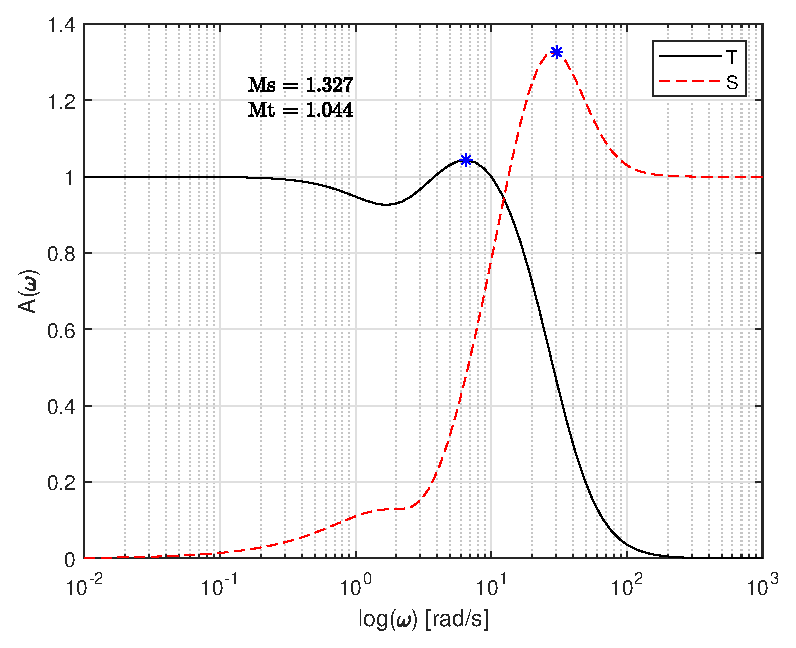
\includegraphics[width=0.46\linewidth]{slike/Ms_Mt_pidc.eps}
		\caption{Prikaz fukcije osetljivosti $S(\omega)$ i komplementarne osetljivosti $T(\omega)$ za PID$\text{c}_1$}
		\label{fig:MsMt_pidc}
	\end{figure}
	
	\begin{figure}[!h]
		\centering
		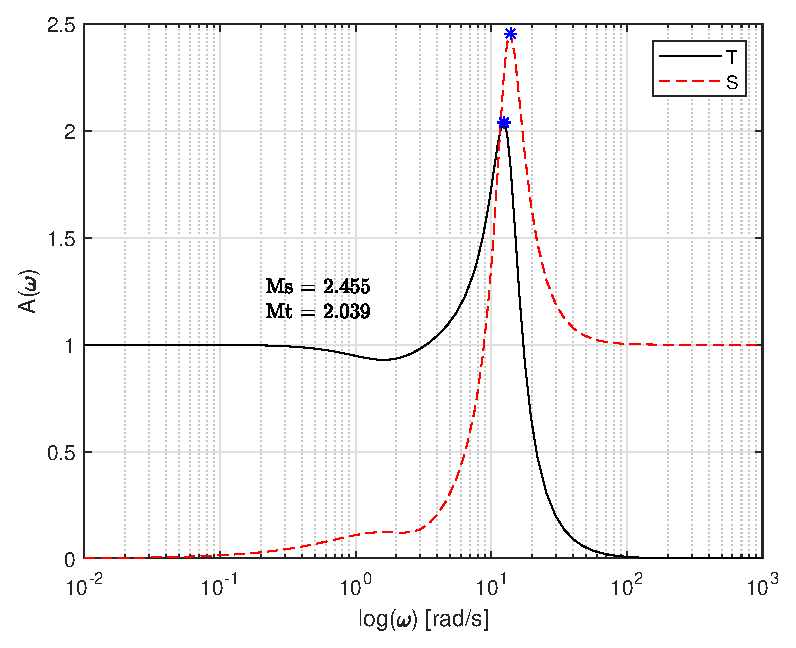
\includegraphics[width=0.46\linewidth]{slike/Ms_Mt_pid.eps}
		\caption{Prikaz fukcije osetljivosti $S(\omega)$ i komplementarne osetljivosti $T(\omega)$ za PID$_{s=0}$}
		\label{fig:MsMt_pid}
	\end{figure}
	
	\begin{figure}[!h]
		\centering
		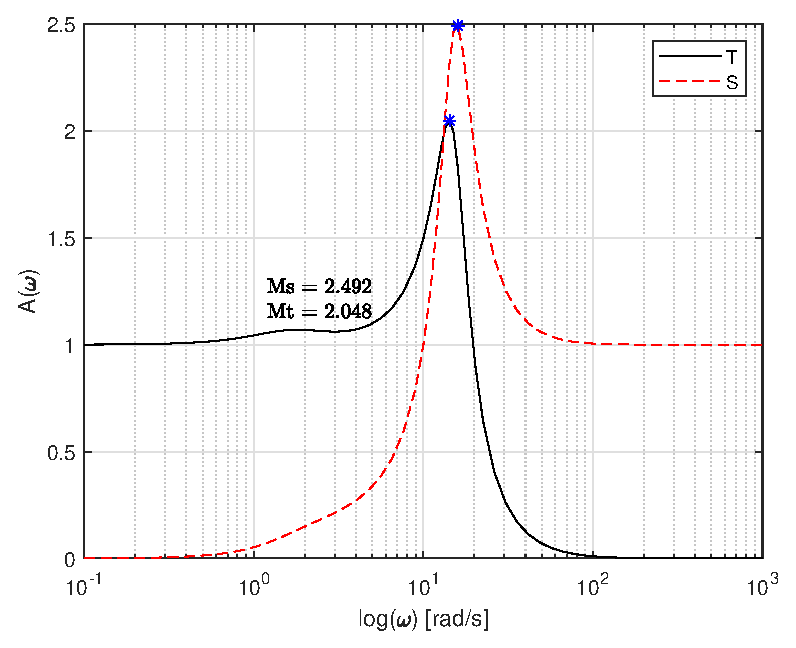
\includegraphics[width=0.46\linewidth]{slike/Ms_Mt_pid_lam.eps}
		\caption{Prikaz fukcije osetljivosti $S(\omega)$ i komplementarne osetljivosti $T(\omega)$ za PID$_{s=\frac{1}{\lambda}}$}
		\label{fig:MsMt_pid_lam}
	\end{figure}
	
	\begin{figure}[!h]
		\centering
		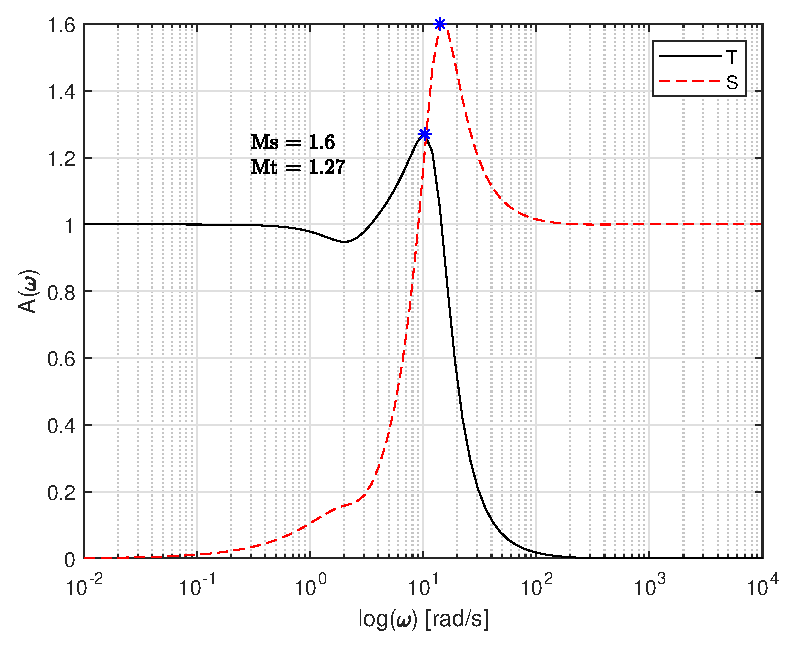
\includegraphics[width=0.6\linewidth]{slike/Ms_Mt_pid_opt.eps}
		\caption{Prikaz fukcije osetljivosti $S(\omega)$ i komplementarne osetljivosti $T(\omega)$ za PID$_{t}$}
		\label{fig:MsMt_pid_opt}
	\end{figure}
	
	\begin{figure}[!h]
		\centering
		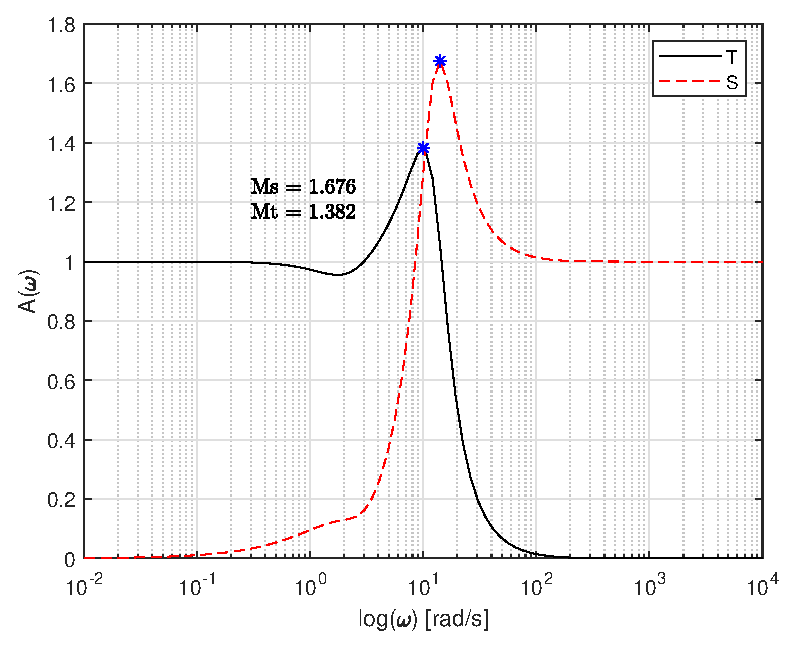
\includegraphics[width=0.6\linewidth]{slike/Ms_Mt_pid_optf.eps}
		\caption{Prikaz fukcije osetljivosti $S(\omega)$ i komplementarne osetljivosti $T(\omega)$ za PID$_{f}$}
		\label{fig:MsMt_pid_optf}
	\end{figure}
	

	\clearpage
	
	\begin{figure}[!h]
		\centering
		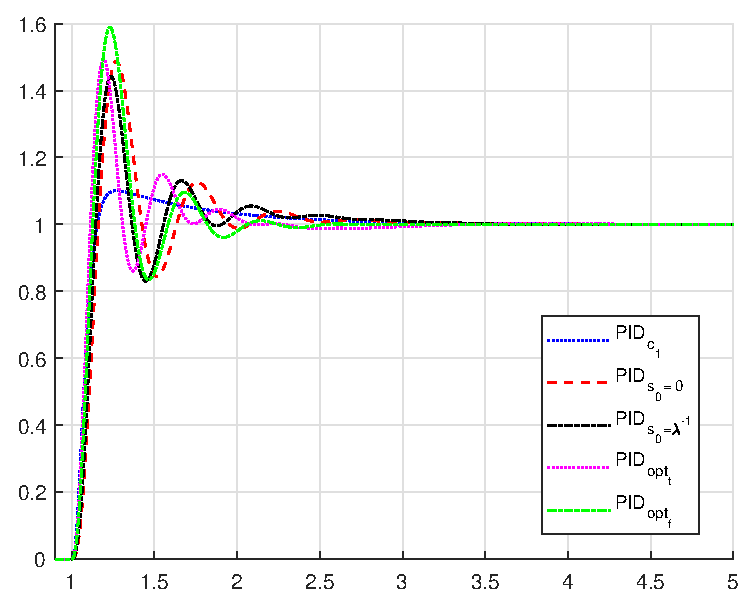
\includegraphics[width=0.6\linewidth]{slike/Pg_comparison_default.eps}
		\caption{Pore\dj{}enje odziva na promenu reference}
		\label{fig:Pg_default}
	\end{figure}
	
	\begin{figure}[!h]
		\centering
		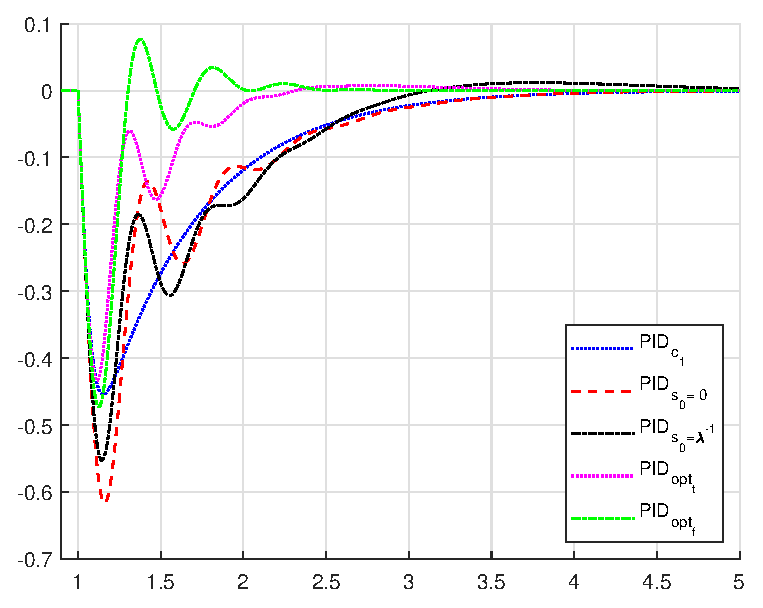
\includegraphics[width=0.6\linewidth]{slike/fm_comparison_default.eps}
		\caption{Pore\dj{}enje odziva na poreme\'caj}
		\label{fig:fm_default}
	\end{figure}
	
	\begin{figure}[!h]
		\centering
		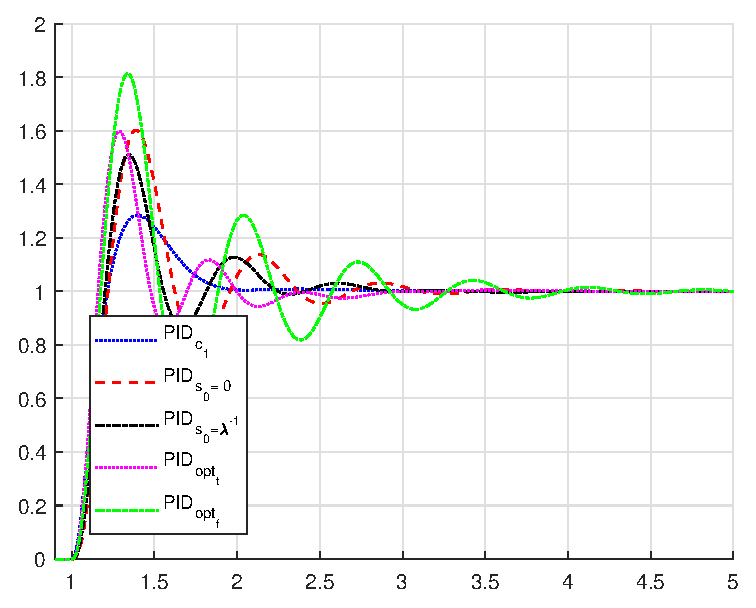
\includegraphics[width=0.6\linewidth]{slike/Pg_comparison_+50.eps}
		\caption{Pore\dj{}enje odziva na promenu reference, parametri uve\'cani za $50\%$}
		\label{fig:Pg_50}
	\end{figure}
	
	\begin{figure}[!h]
		\centering
		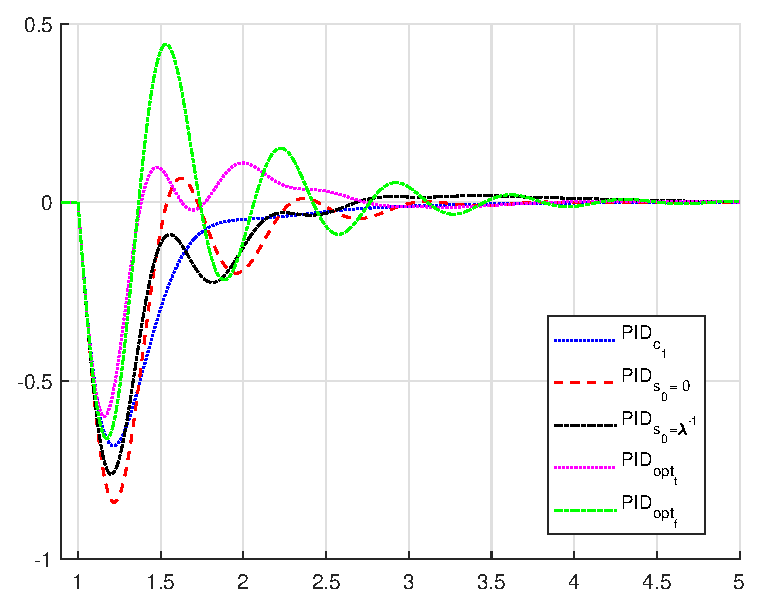
\includegraphics[width=0.6\linewidth]{slike/fm_comparison_+50.eps}
		\caption{Pore\dj{}enje odziva na poreme\'caj, parametri uve\'cani za $50\%$}
		\label{fig:fm_50}
	\end{figure}
	
\begin{figure}[!h]
	\centering
	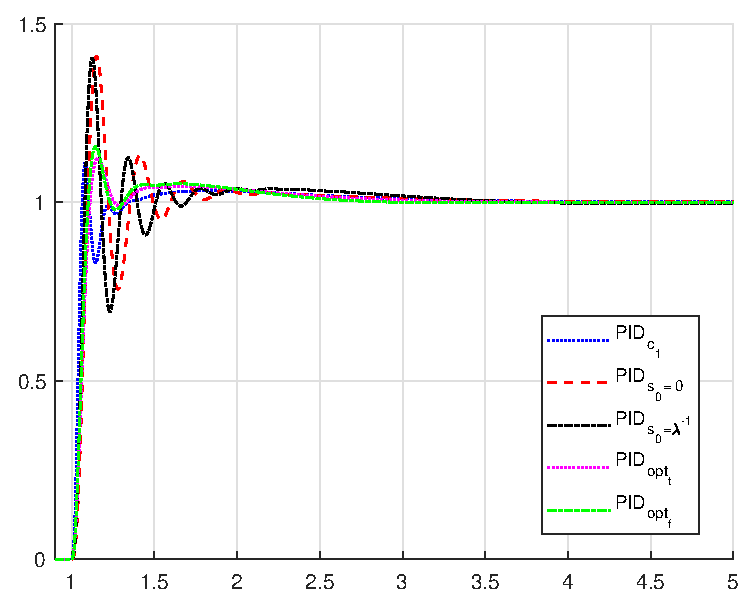
\includegraphics[width=0.6\linewidth]{slike/Pg_comparison_-50.eps}
	\caption{Pore\dj{}enje odziva na promenu reference, parametri smanjeni za $50\%$}
	\label{fig:Pg_-50}
\end{figure}

\begin{figure}[!h]
	\centering
	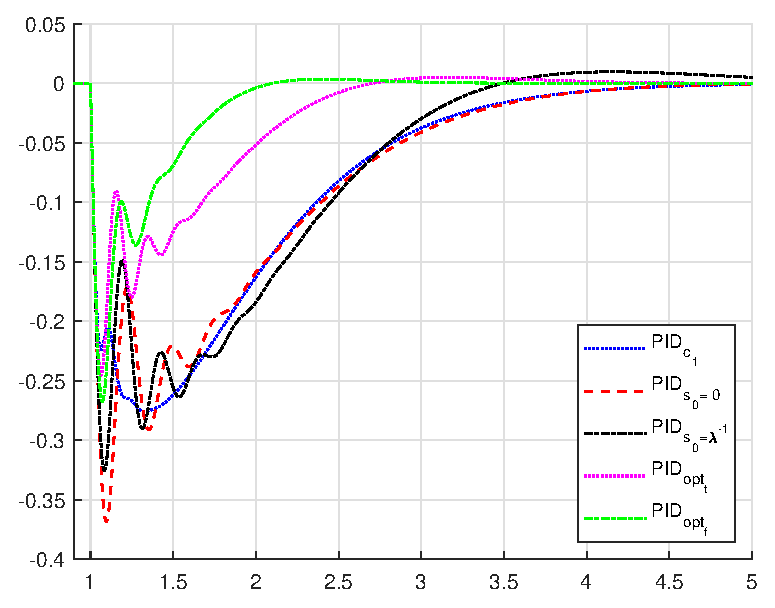
\includegraphics[width=0.6\linewidth]{slike/fm_comparison_-50.eps}
	\caption{Pore\dj{}enje odziva na poreme\'caj,
	parametri smanjeni za $50\%$}
	\label{fig:fm_-50}
\end{figure}

\begin{figure}[!h]
	\centering
	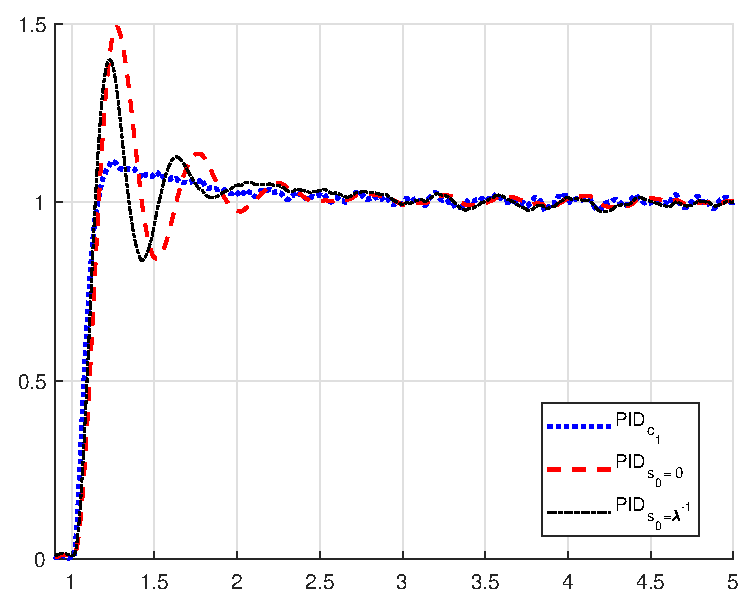
\includegraphics[width=0.6\linewidth]{slike/Pg_comparison_noise.eps}
	\caption{Pore\dj{}enje odziva na promenu reference u prisustvu "suma}
	\label{fig:Pg_noise}
\end{figure}

\begin{figure}[!h]
	\centering
	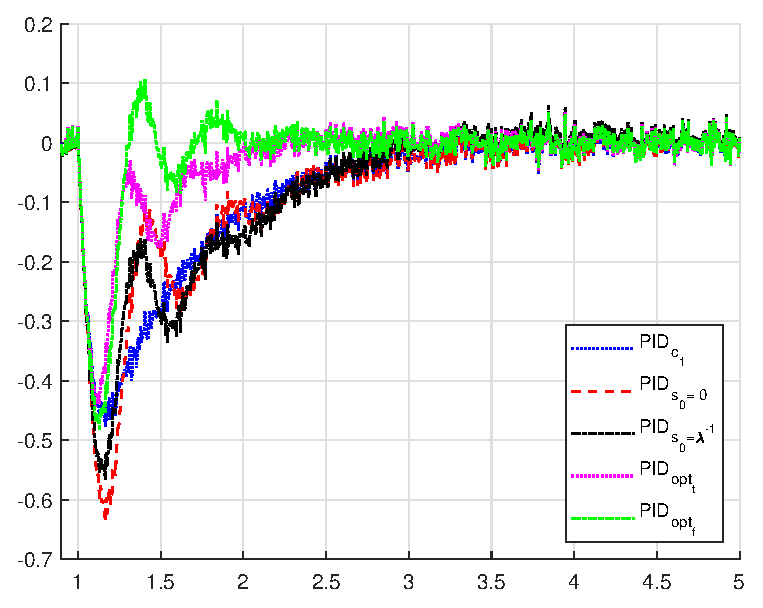
\includegraphics[width=0.6\linewidth]{slike/fm_comparison_noise.eps}
	\caption{Pore\dj{}enje odziva na poreme\'caj,
		u prisustvu "suma}
	\label{fig:fm_noise}
\end{figure}
	
	

	
	
	
	\clearpage
	\subsubsection{Tabelarni prikaz rezultata simulacije}\label{sec:tab}
	
	
	
		\begin{table}[!h]
			\resizebox{.75\textwidth}{!}{%
				\begin{tabular}{lllll}
					\hline
					\multicolumn{5}{c}{Pore\dj{}enje kontrolera, nominalni re"zim} \\ \hline
					& IAE      & IE        & ITAE      & TVd     \\ \hline
					PIDc                              & 67.9387  & -67.9387  & 112.8425  & \textbf{0.9080}  \\ \hline
					PID$_{s_0 = 0}$                   & 67.9410  & -67.9387  & 112.8597  & 1.4884  \\ \hline
					PID$_{s_0 = \frac{1}{\lambda}}$   & 70.0435  & -63.7952  & 120.1797  & 1.3725  \\ \hline
					PID$_t$                           & 28.3491  & -25.4812  & 40.2509   & 1.0999  \\ \hline
					PID$_f$                           & \textbf{22.2346}  & \textbf{-15.3272}  & \textbf{28.0032}   & 1.3082  \\ \hline
				\end{tabular}%
			}
			\label{tab:result_nominal}
		\end{table}
		
	\begin{table}[!h]
		\resizebox{.75\textwidth}{!}{%
			\begin{tabular}{lllll}
				\hline
				\multicolumn{5}{c}{Pore\dj{}enje kontrolera, parametri uve\'cani za $50\%$} \\ \hline
				& IAE      & IE        & ITAE      & TVd     \\ \hline
				PIDc                              & 67.9387  & -67.9387  & 99.8695  & \textbf{1.3648}  \\ \hline
				PID$_{s_0 = 0}$                   & 71.6303  & -67.9387  & 106.2790   & 2.3576  \\ \hline
				PID$_{s_0 = \frac{1}{\lambda}}$   & 73.2516  & -63.7947  & 116.3983   & 1.8473  \\ \hline
				PID$_t$                           & \textbf{39.2494}  & -25.4812  & \textbf{54.8455}   & 1.8282  \\ \hline
				PID$_f$                           & 76.6396  & \textbf{-15.3272}  & 131.9700   & 3.4350  \\ \hline
			\end{tabular}%
		}
		\label{tab:result_+50}
	\end{table}
	
		\begin{table}[!h]
		\resizebox{0.75\textwidth}{!}{%
			\begin{tabular}{lllll}
				\hline
				\multicolumn{5}{c}{Pore\dj{}enje kontrolera, parametri smanjeni za $50\%$} \\ \hline
				& IAE      & IE        & ITAE      & TVd     \\ \hline
				PIDc                              & 67.9387  & -67.9387  & 125.9439  & \textbf{0.5896}  \\ \hline
				PID$_{s_0 = 0}$                   &  67.9606  & -67.9387  & 126.0952   & 1.0112  \\ \hline
				PID$_{s_0 = \frac{1}{\lambda}}$   &  69.0071  & -63.7961  & 130.3229   & 1.0326  \\ \hline
				PID$_t$                           & 27.3529  & -25.4812  & 42.9804    & 0.7117
				  \\ \hline
				PID$_f$                           &  \textbf{16.1923}    & \textbf{-15.3272}  & \textbf{21.4720}   &0.6153  \\ \hline
			\end{tabular}%
		}
		\label{tab:result_-50}
	\end{table}
	
	\begin{table}[!h]
		\resizebox{0.75\textwidth}{!}{%
			\begin{tabular}{lllll}
				\hline
				\multicolumn{5}{c}{Pore\dj{}enje kontrolera u prisustvu "suma} \\ \hline
				& IAE      & IE        & ITAE      & TVd     \\ \hline
				PIDc                              & 81.9753  & -67.7478  & 209.9080  & \textbf{28.8642}  \\ \hline
				PID$_{s_0 = 0}$                   &  82.2774  & -67.6408  &  211.8215`   & 29.0482  \\ \hline
				PID$_{s_0 = \frac{1}{\lambda}}$   &  84.0861  & -63.5301  & 216.8843   & 28.9761  \\ \hline
				PID$_t$                           & 45.5459   & -25.3101   &  149.3210     &  28.9472
				  \\ \hline
				PID$_f$                           &  \textbf{41.1739}    & \textbf{-15.0836}  & \textbf{141.4896}   & 29.0092
				 \\ \hline
			\end{tabular}%
		}
		\label{tab:result_noise}
	\end{table}
		
		
	


	
	\clearpage
	\section{Zaklju"cak}\label{sec:zakljucak}
	
	Rezultati ovog rada jasno ukazuju na prednosti i ograničenja različitih tehnika projektovanja kontrolera u elektroenergetskim sistemima. Velika prednost analiti"ckog projektovanja se ogleda u postojanju podesivih parametara $\lambda$ i $N$. Me\dj{}utim, rezultuju\'ci kontroleri su "cesto vi"seg reda. Ukoliko je neophodno koristiti re"senje na bazi klasi"cnog PID linearizacijom PID$_c$ dobija se PID kontroler prihvatljivih performansi.\\
	
	S druge strane, optimizacija, bilo u vremenskom ili frekvencijskom domenu, nudi znatno efikasnije upravljanje frekvencijom. Optimizovani kontroleri, koji su razvijeni korišćenjem tehnika optimizacije performansi, postigli su bolje rezultate u pogledu smanjenja integrala greške, što ih čini pogodnijim za složene sisteme. Ukoliko je neophodna ve\'ca robustnost to se mo"ze posti\'ci jednostavnom modifikacijom specifikacija otimizacionog problema. \\
	
	Simulacijama je pokazano da su optimizovani kontroleri nadmašili analitički projektovane kontrolere u smislu brzine potiskivanja poreme\'caja. Na osnovu ovih rezultata, može se zaključiti da optimizacija pruža značajne prednosti u situacijama kada su potrebni visoki nivoi performansi i fleksibilnosti u projektovanu sistema upravljanja. \\
	
	Iako su rezultati simulacija pokazali jasne prednosti optimizacije, postoji i nekoliko izazova vezanih za implementaciju ovih metoda u praksi. Naime, proces optimizacije zahteva veći broj simulacija i složenije algoritme, što povećava vreme potrebno za projektovanje kontrolera. Pored toga prona\dj{}eno re"senje ne mora biti globalni optimum. Me\dj{}utim, "cesto je dovoljno imati lokalno optimalnu parametrizaciju razmatranog kontrolera. \\
	
	Još jedno važno pitanje je robustnost kontrolera u prisustvu nesigurnosti u modelu sistema. U ovom radu nije sprovedena dublja analiza robusnosti u smislu najgore kombinacije parametara modela, što predstavlja prostor za dalje unapre\dj{}enje ovog rada. Dalje istraživanje može uključiti implementaciju frakcionog kontrolera i pore\dj{}enje sa implementiranim algoritmima. \\
	
	
	Na kraju, rezultati ovog rada ukazuju na to da iako analitičko projektovanje kontrolera pruža solidnu osnovu za regulaciju frekvencije, optimizacione tehnike nude elegantno rešenje u pogledu performansi i robusnosti. Primena ovih modernih tehnika postaje neophodna u savremenim sistemima upravljanja, gde je od velikog zna"caja ostvariti najbolje mogu\'ce performanse pod ograni"cenjem robustnosti.
	
	
	
	
	
	
	\newpage
	
	\begin{thebibliography}{9}
		\bibitem{inicijalna}
		\emph{ Novel tuning rules for PIDC and PID load frequency controllers considering
			robustness and sensitivity to measurement noise}, Marko Č. Bošković, Tomislav B. Šekara, Milan R. Rapaić
		
		\bibitem{frekvencijski_opt}
		\emph{Optimal tuning of fractional PIDC$^\alpha$ controller in the frequency domain}, Tomislav B. Šekara, Milan R. Rapaić, Mihailo P. Lazarevi\'c
		\bibitem{bele"ske}\emph{Distribuirani i frakcioni sistemi upravljanja - bele"ske sa predavanja}, 
		Tomislav B. Šekara
		
		
	\end{thebibliography}
\end{document}
